\documentclass[12pt letter]{report}
\input{./template/preamble}
\input{./template/macros}
\input{./template/letterfonts}

\title{\Huge{Database Analysis and Design}}
\author{\huge{Madiba Hudson-Quansah}}
\date{}
\usepackage{parskip}
\usepackage{tikz}
\usetikzlibrary{er,positioning}

\setcounter{tocdepth}{4}
\setcounter{secnumdepth}{4}

\begin{document}
\maketitle
\newpage
\pdfbookmark[section]{\contentsname}{too}
\tableofcontents
\pagebreak

\chapter{Entity-Relationship Modelling}

Entity-Relationship modelling is a technique used to model the structure of a database. It is a graphical representation of the entities and their relationships to each other. The entities are the objects that are stored in the database, and the relationships are the connections between the entities. The ER model is used to design the database schema, which is the blueprint for the database.

\section{Entity Types}

\dfn{Entity Type}{
  A group of objects with the same properties, which are identified as having an independent existence. Usually drawn
  on an ER diagram as a rectangle, with the name of the entity type written inside the rectangle.
}

\begin{figure}[htpb]
  \centering
  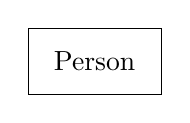
\begin{tikzpicture}[auto,node distance=1.5cm]
    \node[entity] (person) {Person};
  \end{tikzpicture}
\end{figure}

\dfn{Entity Occurrence}{
  A uniquely identifiable object of an entity type.
}

\section{Attributes}

\dfn{Attribute}{
  A property of an entity type. Attributes are the characteristics of the entity type that are stored in the database. Attributes are usually drawn as ovals, with the name of the attribute written inside the oval.
}

\begin{figure}
  \begin{center}
    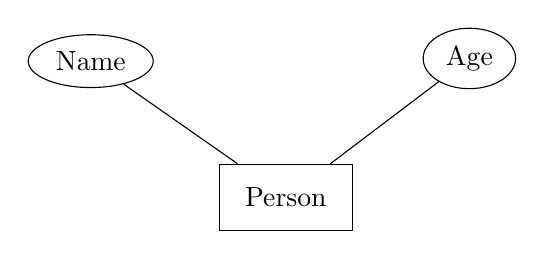
\begin{tikzpicture}[auto,node distance=1.5cm]
      \node[entity] (person) {Person};
      \node[attribute] (name) [above left=of person] {Name};
      \node[attribute] (age) [above right=of person] {Age};

      \path (person) edge node {} (name);
      \path (person) edge node {} (age);
    \end{tikzpicture}
  \end{center}
\end{figure}


\section{Relationships}

\dfn{relationship Type}{
  A set of meaningful associations among entity types. Relationships are usually drawn as diamonds, with the name of the relationship type written inside the diamond.
}

\begin{figure}[htpb]
  \centering
  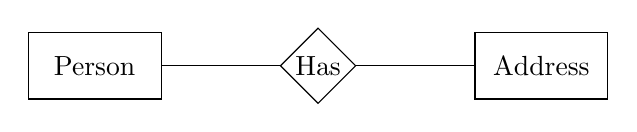
\begin{tikzpicture}[auto,node distance=1.5cm]
    \node[entity] (person) {Person};
    \node[relationship] (has) [right=of person] {Has};
    \node[entity] (address) [right=of has] {Address};

    \path (person) edge node {} (has);
    \path (has) edge node {} (address);
  \end{tikzpicture}
\end{figure}

\chapter{Normalization}

\dfn{Normalization}{
  A technique of producing a set of relations with desirable properties, given the data requirements of an application /
  enterprise.
}

The purpose of normalization is to identify a suitable set of relations that support the data requirements of an
enterprise. The characteristics of a normalized database are:
\begin{itemize}
  \item The minimal number of attributes necessary to support the data requirements of the enterprise.
  \item Attributes with a close logical relationship (i.e. functional dependency) are found in the same relation.
  \item Minimal redundancy, with each attribute represented only once, with important exception of attributes that form
        all or part of foreign keys, which are necessary for joining relations.
\end{itemize}

\section{Data Redundancy and Anomalies}

\section{Functional Dependencies}

\section{Normal Forms}

Three normal forms are commonly used in database design:
\begin{itemize}
  \item First Normal Form (1NF)
  \item Second Normal Form (2NF)
  \item Third Normal Form (3NF)
\end{itemize}

Subsequent normal forms exist, but are not commonly used in practice, for example:
\begin{itemize}
  \item Boyce-Codd Normal Form (BCNF)
  \item Fourth Normal Form (4NF)
  \item Fifth Normal Form (5NF)
\end{itemize}

\subsection{Unnormalized Form (UNF)}

A relation is in Unnormalized Form (UNF) if it contains repeating groups or multi-valued (non-atomic) attributes. In
removing repeating groups in a relation, there are two common approaches:
\begin{itemize}
  \item By entering the appropriate data in the empty columns of rows containing the repeating data.
  \item By placing the repeating data, along with a copy of the original key attributes, in a separate relation.
\end{itemize}

\subsection{First Normal Form (1NF)}

\dfn{First Normal Form}{
  A relation in which the intersection of each row and column contains one and only one value. I.e. complete atomicity.
}

By removing repeating groups, a relation is moved from Unnormalized Form to the First Normal Form (1NF). If a relation
is in 1NF, it:
\begin{itemize}
  \item Has atomic attributes.
  \item Attributes must be of the same data type.
  \item It has a primary key.
  \item There are no repeating attributes.
\end{itemize}


\subsection{Second Normal Form (2NF)}

\dfn{Second Normal Form}{
  A relation that is in 1NF and every non-primary-key attribute is fully functionally dependent on the primary key.
}

Second Normal form applies to relations that have composite keys i.e. the relations with primary comprised of more than
one attribute. A relation with a single attribute primary key is automatically in 2NF.

Normalization from 1NF to 2NF involves:
\begin{itemize}
  \item Removal of partial dependencies.
  \item Creation of new relations for the attributes that are partially dependent on the primary key, where the primary
        key of the original relation is included as a foreign key in the new relation.
\end{itemize}

\subsection{Third Normal Form (3NF)}

\dfn{Third Normal Form}{
  A relation that is in 2NF in which no non-primary-key attribute is transitively dependent on the primary key.
}

\end{document}
